\documentclass[pdftex,a4paper]{scrreprt}
\usepackage[utf8]{inputenc}       
\usepackage[T1]{fontenc}
\usepackage{graphicx}
\usepackage{xcolor}
\usepackage[
	round,	%(defaultage in the main file and \input ) for round parentheses;
	authoryear,% (default) for author-year citations;
	sort,		% orders multiple citations into the sequence in which they 
]{natbib}	
\usepackage{csvsimple}  % read csv files into Latex


\title{Supplemental Materials for the paper: \\Pesticides pollution of small streams in
Germany}
\author{Eduard Szöcs, Marvin Brinke, Bilgin Karaoglan, Ralf B. Schäfer}

\begin{document}
\maketitle

\chapter{Data Cleaning}
Each of more then 30 datasets have been cleaned and homogenized separately, before combing in a common database.
Cleaning steps comprised (Figure~\ref{fig:data_cleaning} gives a graphical overview).

\begin{enumerate}
	\item Structure: Structure has been adjusted to the database structure.
	\item Coordinates: Coordinates have been transformed to a common Coordinate Reference System (DHDN / 3-Grad Gauss-Krüger Zone 3 (EPSG:31467) and duplicates merged.
	\item Chemicals: Chemical names and identifiers have been unified using the webchem package \citep{szocs_webchem:_2016}.
	\item  Identifiers: Unique identifiers have been assigned.
	\item Units: All concentrations have been converted to $\mu g/L$. Values below limit of quantification have be set to zero.
	\item Other meta-data: meta-data has been standardised.
	\item Temporal resolution: The temporal resolution of the database is 1 day. Date below this resolution has been aggregated by maximum.
	\item Validity Checks: Simple rules for validity checks have been implemented (e.g. no negative concentrations).
\end{enumerate}

\begin{figure}
\centering
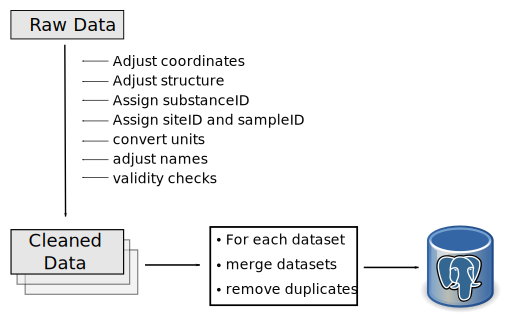
\includegraphics[width = 0.8\textwidth]{data_cleaning}
\caption{Overview on data cleaning steps. After cleaning data has been stored in a relational spatial PostgreSQL database.}
\label{fig:data_cleaning}
\end{figure}

\chapter{Overview on compiled data}

\begin{table}[htbp]
\caption{Overview on chemical samples. Only data from running waters and grab sampling is shown.}
\begin{tabular}{lllrrr}
state\textsuperscript{a} & begin & end & no. sites & no. samples & no. compounds\textsuperscript{b} \\
BW & 2005-01-03 & 2014-10-02 & 118 & 4569 & 127 \\ 
BY & 2006-04-19 & 2013-12-18 & 19 & 297 & 157 \\ 
HE & 2007-01-15 & 2014-12-18 & 68 & 2512 & 144 \\ 
MV & 2005-03-08 & 2014-12-17 & 135 & 1535 & 227 \\ 
NI & 2014-03-24 & 2014-10-13 & 3 & 17 & 226 \\ 
NW & 2005-01-11 & 2015-01-22 & 1320 & 10985 & 204 \\ 
RP & 2005-01-05 & 2013-12-18 & 44 & 1277 & 278 \\ 
SH & 2005-04-26 & 2014-11-26 & 273 & 1419 & 180 \\ 
SL & 2005-01-03 & 2013-12-09 & 6 & 420 & 57 \\ 
SN & 2005-01-02 & 2013-12-18 & 917 & 17052 & 173 \\ 
ST & 2005-01-10 & 2015-03-25 & 46 & 712 & 93 \\ 
TH & 2005-01-31 & 2014-12-10 & 100 & 1441 & 76 \\ \hline
\textbf{Total} & 2005-01-02 & 2015-03-25 & 3049 & 42236 & 484 \\  \hline
\end{tabular}
\\[1em]
\textsuperscript{a}: Abbreviation according to ISO 3166-2:DE .\\
\textsuperscript{b}: Including metabolites.
\label{tab:phch}
\end{table}


\bibliographystyle{apalike}      % basic style, author-year citations
\bibliography{references}

\end{document}